\section{9820 Preliminary Examination}

\begin{problem}
    Let $a$, $b$, $c$ be positive real numbers such that $abc = 36$.

    \begin{enumerate}
        \item Show that $2a + b + 3c \geq 18$.
        \item Deduce the minimum value of \[\frac{4a^2}{b + 3c} + \frac{b^2}{3c + 2a} + \frac{9c^2}{2a + b}\] and find the values of $a$, $b$ and $c$ where this minimum value is attained.
        \item Hence, or otherwise, prove that if $p$, $q$ and $r$ are positive real numbers such that $pqr = 1/36$, then \[\frac1{9p^3 (r + 3q)} + \frac1{36q^3(3p+2r)} + \frac1{4r^3(2q+p)} \geq 9.\]
    \end{enumerate}
\end{problem}
\begin{solution}
    \begin{ppart}
        By AM-GM, \[2a + b + 3c \geq 3 \sqrt[3]{2a \cdot b \cdot 3c} = 3 \sqrt[3]{6abc} = 3\sqrt[3]{6 \cdot 36} = 18.\]
    \end{ppart}
    \begin{ppart}
        By Cauchy-Schwarz, \[\bp{\frac{4a^2}{b+3c} + \frac{b^2}{3c+2a} + \frac{9c^2}{2a+b}}\bs{(b+3c) + (3c+2a) + (2a+b)} \geq \bp{2a+b+3c}^2.\] Thus, 
        \begin{align*}
            \frac{4a^2}{b+3c} + \frac{b^2}{3c+2a} + \frac{9c^2}{2a+b} &\geq \frac{\bp{2a+b+3c}^2}{(b+3c) + (3c+2a) + (2a+b)}\\ 
            &= \frac{2a+b+3c}{2} \geq \frac{18}{2} = 9.
        \end{align*}
        Equality holds when \[\frac{2a}{b+3c} = \frac{b}{3c + 2a} = \frac{3c}{2a + b} \quad \tand \quad 2a = b = 3c,\] i.e. $a = 3$, $b = 6$ and $c = 2$.
    \end{ppart}
    \begin{ppart}
        Take $a = 1/p$, $b = 1/q$ and $c = 1/r$. Note that $abc = 1/pqr = 36$. Using (b), we see that \[\frac{\frac4{p^2}}{\frac1q + \frac3r} + \frac{\frac1{q^2}}{\frac3r + \frac2p} + \frac{\frac9{r^2}}{\frac2p + \frac1q} \geq 9.\] This simplifies to \[\frac{4pqr}{p^3 (r+3q)} + \frac{pqr}{q^3(3p+2r)} + \frac{9pqr}{r^3(2q+p)} \geq 9.\] Recalling that $pqr = 1/36$, we have \[\frac1{9p^3 (r + 3q)} + \frac1{36q^3(3p+2r)} + \frac1{4r^3(2q+p)} \geq 9\] as desired.
    \end{ppart}
\end{solution}

\clearpage
\begin{problem}
    \begin{enumerate}
        \item The variables $x$ and $y$ are related by the differential equation \[\der{y}{x} = \frac{2xy}{x^2 - 2y^2}\] for all $x, y \in \RR$, where $x \neq \sqrt{2} y$. Using the substitution $y = ux$, find the general solution of the differential equation.
        \item Describe geometrically the set of points that satisfy the general solution obtained in part (a).
    \end{enumerate}
\end{problem}
\begin{solution}
    \begin{ppart}
        Note that \[\der{y}{x} = \der{u}{x} x + u.\] Substituting this into the given differential equation, we have \[\der{u}{x} x + u = \frac{2x(ux)}{x^2 - 2(ux)^2}.\] This simplifies to \[\frac{1-2u^2}{u(1+2u^2)} \der{u}{x} = \frac1x.\] Integrating both sides with respect to $x$ gives \[\int \frac{1-2u^2}{u(1+2u^2)} \d u = \int \frac1x \d x.\] The LHS sorts out to \[\int \frac{1-2u^2}{u(1+2u^2)} \d u  = \int \frac1u - \frac{4u}{1 + 2\u^2} \d u = \ln u - \frac{1 + 2u^2} + C_1,\] while the RHS is $\ln x + C_2$. Hence, we have \[\ln \frac{u}{1 + 2u^2} = \ln x + C \implies \frac{u}{1 + 2u^2} = A x.\] Substituting back $u = y/x$, we see that the general solution is \[y = A\bp{x^2 + 2y^2}.\]
    \end{ppart}
    \begin{ppart}
        In the case where $A = 0$, the solution is the horizontal line $y = 0$. Consider then the case where $A \neq 0$. Dividing by $A$ and completing the square, we obtain \[x^2 + 2\bp{y - \frac1{4A}}^2 = \frac1{8A^2}.\] Equivalently, \[\frac{x^2}{\bp{\frac1{\sqrt8 A}}^2} + \frac{\bp{y - \frac1{4A}}^2}{\bp{\frac1{4A}}^2} = 1.\] Thus, the set of points that satisfy the general solution in this case forms the punctured ellipse with centre $(0, 1/4A)$, horizontal radius $1/\sqrt{8} A$ and vertical radius $1/4A$, where $x \neq \sqrt{2}y$.
    \end{ppart}
\end{solution}

\clearpage
\begin{problem}
    Consider 4-by-4 unit square grids where each unit square is either shaded or white. For example, the following diagram illustrates an example of such a grid.

    \begin{center}\tikzsetnextfilename{521}
        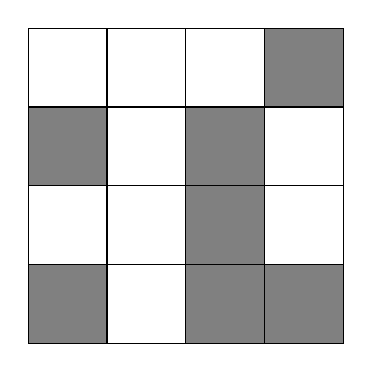
\begin{tikzpicture}
            \draw (0, 0) rectangle (0, 4);
            \draw (1, 0) rectangle (1, 4);
            \draw (2, 0) rectangle (2, 4);
            \draw (3, 0) rectangle (3, 4);
            \draw (4, 0) rectangle (4, 4);

            \draw (0, 0) rectangle (4, 0);
            \draw (0, 1) rectangle (4, 1);
            \draw (0, 2) rectangle (4, 2);
            \draw (0, 3) rectangle (4, 3);
            \draw (0, 4) rectangle (4, 4);

            \draw[fill=gray] (0,0) rectangle (1,1);
            \draw[fill=gray] (2,0) rectangle (3,1);
            \draw[fill=gray] (3,0) rectangle (4,1);
            \draw[fill=gray] (2,1) rectangle (3,2);
            \draw[fill=gray] (2,2) rectangle (3,3);
            \draw[fill=gray] (3,3) rectangle (4,4);
            \draw[fill=gray] (0,2) rectangle (1,3);
        \end{tikzpicture}
    \end{center}

    \begin{enumerate}
        \item \begin{enumerate}
            \item How many possible 4-by-4 unit square grids are there?
            \item How many 4-by-4 unit square grids are there which contain at least one entirely shaded 3-by-3 square?
        \end{enumerate}
        \item Determine the minimum number of shaded unit squares in a 4-by-4 unit square grid to guarantee that it contained at least one entirely shaded 2-by-2 square. Justify your answer.
        \item Define $c_i$, for $i = 1, 2, 3, 4$, to be the number of shaded unit squares in the $i$th column from the left of a given 4-by-4 unit square grid. For example, for the 4-by-4 unit square above, $c_1 = 2$, $c_2 = 0$, $c_3 = 3$, $c_4 = 2$.
        
        How many possible tuples $(c_1, c_2, c_3, c_4)$ are there if the given 4-by-4 unit square grid has
        \begin{enumerate}
            \item exactly 4 shaded-unit squares,
            \item at least 12 shaded unit squares?
        \end{enumerate}
    \end{enumerate}
\end{problem}
\begin{solution}
    \begin{ppart}
        \begin{psubpart}
            Each of the $4^2 = 16$ unit squares are either shaded or not shaded. Thus, the number of possible 4x4 unit square grids is $2^{16} = 65536$.
        \end{psubpart}
        \begin{psubpart}
            Let $S$ be the set of all ways to shade a 4x4 unit square grid.
        
            Label the 4 unit squares in the top-left corner as follows:

            \begin{center}\tikzsetnextfilename{522}
                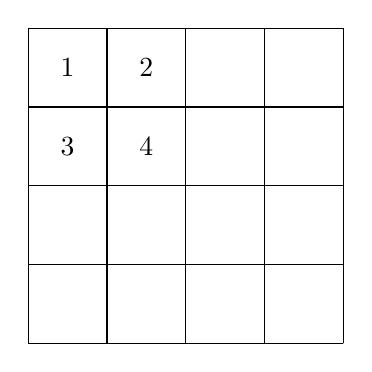
\begin{tikzpicture}
                    \draw (0, 0) rectangle (0, 4);
                    \draw (1, 0) rectangle (1, 4);
                    \draw (2, 0) rectangle (2, 4);
                    \draw (3, 0) rectangle (3, 4);
                    \draw (4, 0) rectangle (4, 4);

                    \draw (0, 0) rectangle (4, 0);
                    \draw (0, 1) rectangle (4, 1);
                    \draw (0, 2) rectangle (4, 2);
                    \draw (0, 3) rectangle (4, 3);
                    \draw (0, 4) rectangle (4, 4);

                    \node at (0.5, 3.5) {1};
                    \node at (1.5, 3.5) {2};
                    \node at (0.5, 2.5) {3};
                    \node at (1.5, 2.5) {4};
                \end{tikzpicture}
            \end{center}

            Let $A_i$ be the set of all ways to shade a 4x4 unit square grid without shading the 3x3 square with square $i$ as its top-left corner, where $1 \leq i \leq 4$.

            For $i = 1, 2, 3, 4$, we have 7 available unit squares to shade, so $\abs{A_i} = 2^7$.

            In the case of two intersecting sets, we have two cases:

            Firstly, if the two shaded 3x3 squares are adjacent to each other, then there are four available unit squares to shade:

            \begin{center}\tikzsetnextfilename{523}
                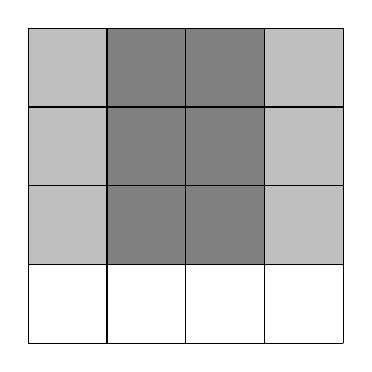
\begin{tikzpicture}
                    \draw[fill=gray!50] (0,1) rectangle (1,4);

                    \draw[fill=gray] (1,1) rectangle (3,4);

                    \draw[fill=gray!50] (3,1) rectangle (4,4);

                    \draw (0, 0) rectangle (0, 4);
                    \draw (1, 0) rectangle (1, 4);
                    \draw (2, 0) rectangle (2, 4);
                    \draw (3, 0) rectangle (3, 4);
                    \draw (4, 0) rectangle (4, 4);

                    \draw (0, 0) rectangle (4, 0);
                    \draw (0, 1) rectangle (4, 1);
                    \draw (0, 2) rectangle (4, 2);
                    \draw (0, 3) rectangle (4, 3);
                    \draw (0, 4) rectangle (4, 4);
                \end{tikzpicture}
            \end{center}
            
            Thus, \[\abs{A_1 \cap A_2} = \abs{A_2 \cap A_3} = \abs{A_3 \cap A_4} = \abs{A_4 \cap A_1} = 2^4.\]

            Secondly, if the two shaded 3x3 squares are not adjacent to each other (i.e. diagonally across each other), then there are 2 available unit squares to shade:

            \begin{center}\tikzsetnextfilename{524}
                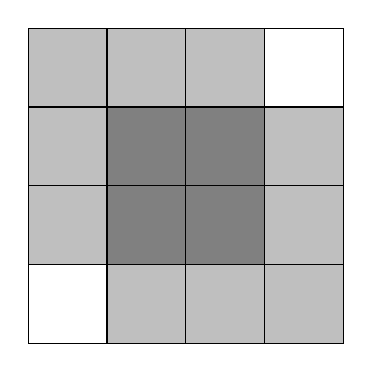
\begin{tikzpicture}
                    \draw[fill=gray!50] (0,1) rectangle (1,4);
                    \draw[fill=gray!50] (1,3) rectangle (3,4);

                    \draw[fill=gray] (1,1) rectangle (3,3);

                    \draw[fill=gray!50] (1,0) rectangle (4,1);
                    \draw[fill=gray!50] (3,1) rectangle (4,3);

                    \draw (0, 0) rectangle (0, 4);
                    \draw (1, 0) rectangle (1, 4);
                    \draw (2, 0) rectangle (2, 4);
                    \draw (3, 0) rectangle (3, 4);
                    \draw (4, 0) rectangle (4, 4);

                    \draw (0, 0) rectangle (4, 0);
                    \draw (0, 1) rectangle (4, 1);
                    \draw (0, 2) rectangle (4, 2);
                    \draw (0, 3) rectangle (4, 3);
                    \draw (0, 4) rectangle (4, 4);
                \end{tikzpicture}
            \end{center}
            
            Thus, \[\abs{A_1 \cap A_4} = \abs{A_2 \cap A_3} = 2^2.\]

            In the case of three intersecting sets, there will always only be one available unit square to shade, so $\abs{A_i \cap A_j \cap A_k} = 2^1$ for distinct $1 \leq i, j, k \leq 3$. Lastly, there is only one way to shade all four 3x3 squares, hence $\abs{A_1 \cap A_2 \cap A_3 \cap A_4} = 1$.

            Finally, by the Principle of Inclusion-Exclusion, the number of 4-by-4 unit square grids that contain at least one entirely shaded 3-by-3 square is given by
            \begin{align*}
                \abs{A_1 \cup A_2 \cup A_3 \cup A_4} &= \binom{4}{1} \cdot 2^7 - \bp{4 \cdot 2^4 + 2 \cdot 2^2} + \binom43 \cdot 2^1 - 1\\
                &= 447.
            \end{align*}
        \end{psubpart}
    \end{ppart}
    \begin{ppart}
        We claim that we need to shade a minimum of 13 unit squares to guarantee a shaded 2x2 square. Note that 12 unit squares do not work due to the following construction:

        \begin{center}\tikzsetnextfilename{525}
            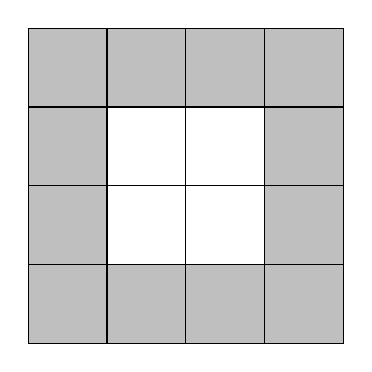
\begin{tikzpicture}
                \draw[fill=gray!50] (0,0) rectangle (4,4);
                \draw[fill=white] (1,1) rectangle (3,3);

                \draw (0, 0) rectangle (0, 4);
                \draw (1, 0) rectangle (1, 4);
                \draw (2, 0) rectangle (2, 4);
                \draw (3, 0) rectangle (3, 4);
                \draw (4, 0) rectangle (4, 4);

                \draw (0, 0) rectangle (4, 0);
                \draw (0, 1) rectangle (4, 1);
                \draw (0, 2) rectangle (4, 2);
                \draw (0, 3) rectangle (4, 3);
                \draw (0, 4) rectangle (4, 4);
            \end{tikzpicture}
        \end{center}

        We now show that 13 shaded squares is minimal. Consider distributing 13 shaded squares to four 2x2 squares, each in one corner. By the pigeonhole principle, at least one 2x2 square will receive $\ceil{13/4} = 4$ shaded squares. This means that we have a completely shaded 2x2 square, so we are done.
    \end{ppart}
    \begin{ppart}
        \begin{psubpart}
            We have the equation $c_1 + c_2 + c_3 + c_4 = 4$, where $c_i \in \NN_0$ for $1 \leq i \leq 4$. By stars-and-bars, there are $\binom{4+3}{3} = 35$ solutions.
        \end{psubpart}
        \begin{psubpart}
            It suffices to count the number of grids that have at most 4 white unit-squares. Let $d_i$ be the number of white squares in the $i$ column from the left. Then we have $d_1 + d_2 + d_3 + d_4 \leq 4$. Introduce the dummy variable $d_5 \geq 0$ to convert the inequality into an equality: \[d_1 + d_2 + d_3 + d_4 + d_5 = 4.\] By stars-and-bars, there are $\binom{4+4}{4} = 70$ solutions.
        \end{psubpart}
    \end{ppart}
\end{solution}

\begin{problem}
    Let $S$ be the set of all integers from 1 to $n$ and $T$ the set of all subsets of $S$, including the empty set $\varnothing$ and $S$ itself.

    \begin{enumerate}
        \item Explain why $\abs{T} = 2^n$.
    \end{enumerate}

    The sets $A_1$ and $A_2$, which are not necessarily distinct, are chosen randomly and independently from the $2^n$ subsets in $T$.

    \setcounter{enumi}{1}
    \begin{enumerate}
        \item In this part of the question, we will calculate $\P{A_1 \cap A_2 = \varnothing}$ in two ways.
        \begin{enumerate}
            \item Let $i$ be an integer such that $0 \leq i \leq n$. Show that $\P{i \notin A_1 \cap A_2} = 3/4$.
            \item Hence, find $\P{A_1 \cap A_2 = \varnothing}$.
            \item Let $k$ be an integer such that $0 \leq k \leq n$. Find $\P{A_1 \cap A_2 = \varnothing}{\abs{A_1} = k}$.
            \item Deduce that \[\sum_{k = 0}^n \binom{n}{k} \frac1{2^{n+k}} = \bp{\frac34}^n.\]
        \end{enumerate}
        \item \begin{enumerate}
            \item Let $k$ be an integer such that $0 \leq k \leq n$. Find $\P{\abs{A_1 \cap A_2} = k}$.
            \item Find $\E{\abs{A_1 \cap A_2}}$.
        \end{enumerate}
    \end{enumerate}
\end{problem}
\begin{solution}
    \begin{ppart}
        When creating a subset $A \subset S$, we have two choices for each element $i \in S$: either $i \in A$ or $i \notin A$. Since there are a total of $n$ elements, by the multiplication principle, there are $2^n$ ways to construct a subset of $A$, i.e. $\abs{T} = 2^n$.
    \end{ppart}
    \begin{ppart}
        \begin{psubpart}
            Note that
            \begin{align*}
                \P{i \notin A_1 \cap A_2} &= 1 - \P{i \in A_1 \cap A_2}\\
                &= 1 - \P{i \in A_1} \P{i \in A_2}\\
                &= 1 - \frac12 \cdot \frac12\\
                &= \frac34,
            \end{align*}
            where we used the independence of $A_1$ and $A_2$ in the second equality.
        \end{psubpart}
        \begin{psubpart}
            Using the above result, we have \[\P{A_1 \cap A_2 = \varnothing} = \prod_{i = 1}^n \P{i \notin A_1 \cap A_2} = \prod_{i = 1}^n \frac34 = \bp{\frac34}^n.\]
        \end{psubpart}
        \begin{psubpart}
            Each of the $n-k$ elements not in $A_1$ have two choices: to be or not to be in $A_2$. By the multiplication principle, there are $2^{n-k}$ subsets disjoint to $A_1$. Thus, \[\P{A-1 \cap A_2 = \varnothing}{\abs{A_1} = k} = \frac{2^{n-k}}{2^n}.\]
        \end{psubpart}
        \begin{psubpart}
            Observe that there are $\binom{n}{k}$ ways to construct a subset of size $k$, so \[\P{\abs{A_1} = k} = \frac{\binom{n}{k}}{2^n}.\] The given sum can hence be written as \[\sum_{k = 0}^n \binom{n}{k} \frac1{2^{n+k}} = \sum_{k = 0}^n 2^{-k} \cdot \frac{\binom{n}{k}}{2^n} = \sum_{k = 0}^n \P{A_1 \cap A_2 = \varnothing}{\abs{A_1} = k} \P{\abs{A_1} = k}.\] By the law of total probability, this is simply \[\P{A_1 \cap A_2 = \varnothing} = \bp{\frac34}^n.\]            
        \end{psubpart}
    \end{ppart}
    \begin{ppart}
        \begin{psubpart}
            Pick the $k$ elements common to both $A_1$ and $A_2$. There are $\binom{n}{k}$ ways to do so. Let the elements in common be $a_i$, where $1 \leq i \leq k$. Similarly, let the elements not in common be $b_j$, where $1 \leq j \leq n-k$. Then \[\P{\abs{A_1 \cap A_2} = k} = \binom{n}{k} \prod_{i = 1}^k \P{a_i \in A_1 \cap A_2} \prod_{j = 1}^{n-k} \P{b_i \notin A_1 \cap A_2} = \binom{n}{k} \bp{\frac14}^k \bp{\frac34}^{n-k}.\]
        \end{psubpart}
        \begin{psubpart}
            The above result implies that $\abs{A_1 \cap A_2} \sim \Binom{n}{1/4}$. Thus, $\E{\abs{A_1 \cap A_2}} = n/4$.
        \end{psubpart}
    \end{ppart}
\end{solution}

\begin{problem}
    \begin{enumerate}
        \item Let $f(x)$ be a polynomial with integer coefficients.
        \begin{enumerate}
            \item For integers $\a$ and $\b$, show that $f(x) - f(\a)$ has a factor of $x - \a$. Hence, or otherwise, show that \[f(\b) - f(\a) \equiv 0 \pmod{\b-\a}.\]
            \item Deduce that there does not exist a polynomial $f$ with integer coefficients such that $f(1) = 2$ and $f(3) = 5$.
            \item Explain why there does not exist a polynomial $f$ with integer coefficients such that $f(1) = 0$, $0 < f(2025) < 2024$.
        \end{enumerate}
        \item A monic degree $n$ polynomial where the coefficient of $x^n$ is 1. Let $p$ be an odd prime. Let $h(x)$ be a monic degree $n$ polynomial with integer coefficients. We call an integer $\g$ a root modulo $p$ of $h(x)$ if $h(\g) \equiv 0 \pmod{p}$. Moreover, if $\a$ and $\b$ are roots modulo $p$ of $h(x)$ such that $\a \not\equiv \b \pmod{p}$, we call the integers $\a$ and $\b$ incongruent.
        \begin{enumerate}
            \item Find two incongruent roots modulo 7 for $x^2 + x + 1$.
            \item For $n \geq 1$, show that if $\g$ is a root modulo $p$ of $h(x)$, then there exists a monic degree $n-1$ polynomial $h_0(x)$ with integer coefficients such that \[h(x) \equiv (x-\g) h_0(x) \pmod{p}.\]
            \item Prove, by induction, that any monic degree $n$ polynomial $h(x)$ has at most $n$ incongruent roots modulo $p$ for $n \geq 0$.
        \end{enumerate}
    \end{enumerate}
\end{problem}
\begin{solution}
    \begin{ppart}
        \begin{psubpart}
            Since $f(\a) - f(\a) = 0$, by the Factor Theorem, it follows that $x - \a$ is a factor of $f(x) - f(\a)$. Hence, we may write \[f(x) - f(\a) = (x-\a) Q(x)\] for some polynomial $Q(x)$ with integer coefficients. Taking $x = \b$, we have \[f(\b) - f(\a) = (\b - \a) Q(\b) \equiv 0 \pmod{\b - \a}.\]
        \end{psubpart}
        \begin{psubpart}
            Suppose for a contradiction that there exists such a polynomial $f$. Then \[f(3) - f(1) = 5 -2 = 3 \equiv 1 \pmod{3-1}.\] But $1 \not\equiv 0 \pmod{2}$, contradicting the result in (a)(i). Thus, such an $f$ cannot exist.
        \end{psubpart}
        \begin{psubpart}
            Suppose for a contradiction that there exists such a polynomial $f$. By (a)(i), \[f(2024) = f(2025) - f(1) \equiv 0 \pmod{2024}.\] But $0 < f(2024) < 2024$, so $f(2024)$ cannot be a multiple of 2024, a contradiction. Thus, such an $f$ cannot exist.
        \end{psubpart}
    \end{ppart}
    \begin{ppart}
        \begin{psubpart}
            Note that \[2^2 + 2 + 1 = 4^2 + 4 + 1 \equiv 0 \pmod{7}.\] Since $2 \not\equiv 4$ modulo 7, by definition, 2 and 4 are incongruent roots modulo 7 for $x^2 + x + 1$.
        \end{psubpart}
        \begin{psubpart}
            We have $h(\g) \equiv 0 \pmod{p}$, so $h(\g) = kp$ for some integer $k$. By the remainder theorem, there exists some polynomial $Q(x)$ with integer coefficients such that $h(x) = (x-\g) Q(x) + kp$. Reducing modulo $p$, \[h(x) \equiv (x-\g) Q(x) \pmod{p}.\]

            We now check that $Q(x)$ satisfies the postulated properties. Since $\Deg h(x) = n$, it follows that $\Deg Q(x) = n-1$. Further, on comparing coefficients of $x^n$, we see that $Q(x)$ must be monic. Thus, $h_0(x) = Q(x)$.
        \end{psubpart}
        \begin{psubpart}
            Let $P(n)$ be the statement ``any monic degree $n$ polynomial $h(x)$ has at most $n$ incongruent roots modulo $p$''.

            Consider the base case $n = 0$. The only monic degree 0 polynomial is $h(x) = 1$, which has no roots modulo any prime $p$. Thus, $P(0)$ is true.

            Suppose $P(k-1)$ is true for some positive integer $k$. Let $h(x)$ be a monic degree $k$ polynomial with integer coefficients. If $h(x)$ has no roots modulo $p$, we see that $P(k)$ holds, and we are done. Consider then the case where $h(x)$ has a root modulo $p$. Let this root be $\ep$. From (b)(ii), there exists a monic degree $k-1$ degree polynomial $h_0(x)$ with integer coefficients such that \[h(x) \equiv (x-\ep) h_0(x).\] By our inductive hypothesis, $h_0(x)$ has at most $k-1$ incongruent roots modulo $p$. Say there are $j \leq k-1$ incongruent roots. Label these roots $\ep_i$, where $1 \leq i \leq j$.

            If $\ep = \ep_i$ for some $1 \leq i \leq j$, then the only incongruent roots of $h(x)$ are $\ep_i$ for $1 \leq i \leq j$. Since there are $j \leq k-1 \leq k$ such roots, it follows that $P(k)$ is true.

            Else, if $\ep \neq \ep_i$ for all $1 \leq i \leq j$, the $h(x)$ has $j+1 \leq k$ incongruent roots, namely $\ep_1, \dots, \ep_j$ and $\ep$. Thus, $P(k)$ is true.

            In all cases, $P(k)$ is true. Thus, $P(k-1) \implies P(k)$.

            Since $P(0)$ is true and $P(k-1) \implies P(k)$ for all positive integers $k$, by the Principle of Mathematical Induction, it follows that $P(n)$ is true for all non-negative integers $n$. That is, any monic degree $n$ polynomial $h(x)$ has at most $n$ incongruent roots modulo $p$ for $n \geq 0$.
        \end{psubpart}
    \end{ppart}
\end{solution}

\begin{problem}
    \begin{center}
        \textbf{\underline{On the Irrationality of $\pi$}}
    \end{center}
    We denote $f^{(k)}(x)$ to be the $k$th derivative of $f(x)$ with respect to $x$ and $f^{(0)}(x) = f(x)$.

    A number is called rational if it can be simplified to the form $a/b$ where $a$ is an integer and $b$ is a positive integer where $a$ and $b$ do not share any prime factors. A number is called irrational if it is not a rational number. For example, the numbers $0$, $1$, $4/3$, $-39/13 = -3$ are rational numbers but $\sqrt2$ and $\pi$ are not.

    However, showing that $\pi$ is irrational is not trivial.

    In 1947, the Canadian-American mathematician Ivan Morton Niven produced an elementary yet elegant proof that $\pi$ is irrational. His methods could be traced back to French mathematician Charles Hermite's 1873 paper on proving the irrationality of $\e^r$, where $r$ is a rational number. We will investigate a modified version of Niven's proof of the irrationality of $\pi$.

    We suppose that $\pi = a/b$ for positive integers $a, b$ for contradiction.

    In his proof, for each positive integer $n$, Niven considered the polynomial \[f(x) = \frac{x^n (a-bx)^n}{n!} = \frac{b^n \bs{x(\pi-x)}^n}{n!}.\] Using binomial expansion, we can write this polynomial in the form \[f(x) = \frac1{n!} \sum_{r = n}^{2n} c_r x_r,\] where $c_r$ are integers for all $r$.

    By considering the expansion, we can show that $f^{(k)}(0)$ is an integer for $0 \leq k \leq 2n$. This would then imply that $f^{(k)}(\pi)$ is an integer for $0 \leq k \leq 2n$ as well.

    Niven also defined another function $F(x)$ as \[F(x) = f(x) - f^{(2)}(x) + f^{(4)}(x) - \dots + (-1)^{n} f^{(2n)}(x).\] This is carefully chosen so that the identity \[\int_0^\pi f(x) \sin x \d x = F(0) + F(\pi)\] holds for all $n$.

    For $0 < x < \pi$, we have $0 < f(x) < \pi^n m^n / n!$ for some positive real constant $m$. We can then develop the bound \[0 < \int_{0}^{\pi} f(x) \sin x \d x < \frac{2\pi^n m^n}{n!}\] for all $n \geq 1$. It is a known fact that if $\lim_{n \to \infty} u_n = 0$, this implies that for sufficiently large $n$, we have $u_n < 1$. By selecting a sufficiently large $n$, we will attain the required contradiction to prove that $\pi$ is irrational.

    \separator

    In this question, you are asked to prove that $\pi$ is irrational. For the entirety of the question, we will assume that $\pi = a/b$, where $a, b$ are positive integers, for contradiction.

    \begin{enumerate}
        \item \begin{enumerate}
            \item Consider any $c_r$ in the sum \[f(x) = \frac1{n!} \sum_{k = n}^{2n} c_r x^r.\] Briefly explain why $c_r$ is an integer.
            \item Hence, explain why $f^{(k)}(0)$ is an integer for $0 \leq k \leq 2n$.
        \end{enumerate}
        \item By showing that $f(x) = f(\pi - x)$, prove that $f^{(k)}(\pi)$ is an integer for $0 \leq k \leq 2n$.
        \item \begin{enumerate}
            \item Prove that $F''(x) = f(x) - F(x)$.
            \item Deduce that \[\int_0^\pi f(x) \sin x \d x = F(0) + F(\pi).\]
        \end{enumerate}
        \item \begin{enumerate}
            \item Prove that for some positive real constant $m$, $0 < f(x) < \pi^n m^n / n!$ for $0 < x < \pi$.
            \item Hence, show that \[0 < \int_0^\pi f(x) \sin x \d x < \frac{2\pi^n m^n}{n!}.\]
            \item By considering the series expansion of $\e^x$, or otherwise, explain why \[\lim_{n \to \infty} \frac{2\pi^n m^n}{n!} = 0.\]
        \end{enumerate}
        \item Prove that $\pi$ is irrational.
    \end{enumerate}
\end{problem}
\begin{solution}
    \begin{ppart}
        \begin{psubpart}
            By the binomial theorem,
            \begin{align*}
                f(x) &= \frac{1}{n!} x^n (a-bx)^n\\
                &= \frac1{n!} x^n \sum_{r = 0}^n \binom{n}{r} a^{n-r} (-bx)^r\\
                &= \frac1{n!} \sum_{r = n}^{2n} \binom{n}{r-n} a^{2n-r} (-b)^{r-n} x^{r},
            \end{align*}
            Thus, \[c_r = \binom{n}{r-n} a^{2n-r} (-b)^{r-n},\] which is clearly an integer for all $r$.
        \end{psubpart}
        \begin{psubpart}
            For $0 \leq k \leq n-1$, the polynomial $f^{(k)}(x)$ has no constant term, thus $f^{(k)}(0) = 0$. For $n \leq k \leq 2n$, the polynomial $f^{(k)}(x)$ has constant term $k! c_k / n!$ which is an integer since $k \geq n$.
        \end{psubpart}
    \end{ppart}
    \begin{ppart}
        From the definition \[f(x) = \frac{b^n \bs{x(\pi-x)}^n}{n!},\] it is clear that $f(\pi-x) = f(x)$. Differentiating this $k$ times with respect to $x$, we obtain \[(-1)^k f^{(k)}(\pi-x) = f^{(k)}(x),\] so $f^{(k)}(\pi-x)(0) = (-1)^k f^{(k)}(0)$. By (a)(ii), we see that the RHS is an integer for $0 \leq k \leq 2n$, hence the LHS, $f^{(k)}(\pi-x)(0)$, must also be an integer.
    \end{ppart}
    \begin{ppart}
        \begin{psubpart}
            We are given \[F(x) = \sum_{k = 0}^n (-1)^k f^{(2k)}(x).\] Differentiating twice, we get \[F''(x) = \sum_{k = 0}^{n} (-1)^{k+2} f^{(2k+2)}(x) = -\sum_{k = 1}^{n} (-1)^{k} f^{(2k)}(x),\] where we used the fact that $f^{(2k+2)}(x) = 0$ for all $x$, since $f$ has degree $2n < 2n+2$. Thus, \[F(x) + F''(x) = \sum_{k = 0}^n (-1)^k f^{(2k)}(x) -\sum_{k = 1}^{n} (-1)^{k} f^{(2k)}(x) = f^(0)(x) = f(x).\] Rearranging gives $F''(x) = f(x) - F(x)$.
        \end{psubpart}
        \begin{psubpart}
            Integrating by parts twice, we see that \[\int_0^\pi F''(x) \sin x \d x = F(0) + F(\pi) - \int_0^\pi F(x) \sin x \d x.\] Thus, using (c)(i), \[\int_0^\pi f(x) \sin x \d x = \int_0^\pi F(x) \sin x \d x + \int_0^\pi F''(x) \sin x \d x = F(0) + F(\pi).\]
        \end{psubpart}
    \end{ppart}
    \begin{ppart}
        \begin{psubpart}
            Observe that for $0 < x < \pi = a/b$, we have \[0 < x(a-bx) = \frac{a^2}{4b} - b\bp{x - \frac{a}{2b}}^2 \leq \frac{a^2}{4b} = \frac{\pi a}{4}.\] Hence, \[f(x) = \frac{\bs{x(a-bx)}^n}{n!} \leq \frac1{n!} \bp{\frac{a\pi}{4}}^n < \frac{\pi^n a^n}{n!},\] so $m = a$.
        \end{psubpart}
        \begin{psubpart}
            From the (d)(i), it follows that \[0 < f(x) \sin x < \frac{\pi^n a^n}{n!} \sin x\] for $0 < x < \pi$. Thus, \[0 < \int_0^\pi f(x) \sin x \d x < \frac{\pi^n a^n}{n!} \int_0^\pi \sin x \d x = \frac{2\pi^n a^n}{n!}.\]
        \end{psubpart}
        \begin{psubpart}
            Note that $\pi^n m^n / n!$ is the $n$th term in the series expansion of $\e^{\pi m}$. Since $\e^{\pi m}$ converges, its $n$th term must tend to 0 as $n \to \infty$. Thus, \[\lim_{n \to \infty} \frac{2\pi^n m^n}{n!}  = 2\lim_{n \to \infty} \frac{\pi^n m^n}{n!} = 0.\]
        \end{psubpart}
    \end{ppart}
    \begin{ppart}
        By (a)(ii), \[F(0) = \sum_{k = 0}^n (-1)^k f^{2k}(0) \in \ZZ.\] Likewise, by (b), $F(\pi) \in \ZZ$. Thus, by (c)(ii), \[\int_0^\pi f(x) \sin x \d x \in \ZZ.\] By (d)(iii), we can take $n$ sufficiently large, so that $2\pi^n m^n/n!$ is arbitrarily close to 0. Applying the bounds given by (d)(ii), \[0 < \int_0^\pi f(x) \sin x \d x < \frac{2\pi^n m^n}{n!} < 1,\] so there is an integer in the interval $(0, 1)$, a contradiction. Thus, our assumption that $\pi$ is rational is flawed, so $\pi$ is irrational.
    \end{ppart}
\end{solution}